% Created 2023-08-26 Sat 15:05
% Intended LaTeX compiler: pdflatex
\documentclass[11pt,a4paper,final]{article}
\usepackage[a4paper, total={7in, 10in}]{geometry}
\usepackage{algorithm2e}
\usepackage{booktabs}
\usepackage{subcaption}
\usepackage{graphicx}
\usepackage{tikz}
\usepackage[utf8]{inputenc}
\usepackage[T1]{fontenc}
\usepackage{graphicx}
\usepackage{longtable}
\usepackage{wrapfig}
\usepackage{rotating}
\usepackage[normalem]{ulem}
\usepackage{amsmath}
\usepackage{amssymb}
\usepackage{capt-of}
\usepackage{hyperref}
\usepackage{lipsum}                         % Dummy filler text
\usepackage{amsfonts}                       % Cool math fonts
\usepackage{multicol}                       % Add capability to make columns
\usepackage{hyperref}                       % Cool clean hyperlinks
\setlength\parindent{0pt}                   % No indent for paragraphs
\usetikzlibrary{arrows.meta}                % Arrows for tikz
\renewcommand*{\sectionautorefname}{Section}
\renewcommand*{\subsectionautorefname}{Subsection}
\renewcommand*{\subsubsectionautorefname}{Subsubsection}
\renewcommand*{\paragraphautorefname}{Paragraph}
\renewcommand*{\algorithmautorefname}{Algorithm}
\newcommand{\Or}{\textbf{ or }}
\renewcommand*{\And}{\textbf{ and }}
\newcommand\mycommfont[1]{\footnotesize\ttfamily\textcolor{gray}{#1}}
\newcommand{\T}{\mathcal{T}}                % To make it clear the difference
\newcommand{\Tau}{T}                        % between Tau and T
\newcommand{\AC}{AC(u, d, v, \eta)}         % Set the parameters for AC once
\newcommand{\PC}{PC(u, d, v)}               % Set the parameters for PC once
\newcommand{\ACi}{AC(u_i, d_i, v_i, \eta_i)}% Set the parameters for AC once
\newcommand{\PCi}{PC(u_i, d_i, v_i)}        % Set the parameters for PC once
\newcommand{\Not}{\textbf{not }}            % Custom `not' operator
\newcommand{\visit}{(b_i, a_i, e_i, u_i, d_i, v_i, \eta_i, \xi_i)}
\newcommand{\I}{\mathbb{I}}                 % Set of visit tuples
\newcommand{\C}{\mathbb{C}}                 % Charger availability information
\newcommand{\U}{\mathcal{U}}                % Uniform distribution
\newcommand{\Sol}{\mathbb{S}}               % A shorthand for visit tuple
\newcommand{\M}{\mathbb{M}}                 % A shorthand for the metadata
\newcommand{\Hd}{\mathbb{H}}                % Set of discrete times
\newcommand{\Nu}{\mathcal{V}}               % Draw a nice Nu
\newcommand{\Iset}{\mathcal{I}}             % Set of visits 1-I
\newcommand{\Isetinit}{\mathcal{I}_0}       % Set of visits inital visits
\newcommand{\Isetfinal}{\mathcal{I}_f}      % Set of visits final visits
\newcommand{\Bset}{\mathcal{B}}             % Set of visits 1-B
\newcommand{\Qset}{\mathcal{Q}}             % Set of visits 1-Q
\newcommand{\Jset}{\mathcal{J}}             % Set of visits 1-J
\newcommand{\Jsetq}{\mathbb{J}}             % Set of visits 1-J for queue active times
\newcommand{\Hset}{\mathcal{H}}             % Set of visits 1-H
\author{Alexander Brown}
\date{\today}
\title{Bus Charging Schedule Simulated Annealing with MILP Constraints}
\hypersetup{
 pdfauthor={Alexander Brown},
 pdftitle={Bus Charging Schedule Simulated Annealing with MILP Constraints},
 pdfkeywords={},
 pdfsubject={},
 pdfcreator={Emacs 29.1 (Org mode 9.6.7)}, 
 pdflang={English}}
\begin{document}

\maketitle
\tableofcontents

\parskip 3mm                                % Set the vetical space between paragraphs
\let\ref\autoref                            % Redifine `\ref` as `\autoref` because lazy
\SetCommentSty{mycommfont}                  % Set the comment color

\section{Introduction}
\label{sec:introduction}
This document outlines a Simulated Annealing (SA) approach to the bus charging scheduling problem that utilizes Mixed
Integer Linear Programming (MILP) constraints to determine feasible charging schedules. The problem involves generating
an optimal charging schedule for a fleet of Battery Electric Buses (BEBs) based on a set of routes and a mix of fast and
slow chargers. The aim is to minimize both the consumption cost (amount of electricity used over a certain time) and the
demand cost (rate at which electricity is being used) while ensuring that the buses maintain sufficient charge to
complete their workday without delays.

The SA algorithm is introduced and constrained by a set of MILP constraints derived from the Position Allocation Problem
(PAP) to ensure the validity of proposed charging schedules. Objective functions describing consumption cost and demand
cost are used to minimize power consumption and total cost of using the BEBs.
\section{Problem Description}
\label{sec:problem-description}
It is assumed that there are a total of \(I\) visits to the station by \(B\) buses. There are a total of \(Q\) queues for the
bus at the station. Let \(\mathcal{Z}\) be the set of integers, given a set of bus arrivals to a charging station \(i \in \{1,..., I\}
= \Iset \subset \mathcal{Z}\) with a set of chargers to be queued \(q \in \{1,..., Q\} = \Qset \subset \mathcal{Z}\) where the bus is indicated by an
identification number \(b \in \{1,..., B\} = \Bset \subset \mathcal{Z}\). Each bus arrival, \(i\), can be represented by the tuple: \(\visit\),
in which the ordered elements denote the bus identification number, \(b_i\), arrival time to the station, \(a_i\), departure
time from the station, \(e_i\), time to start charging, \(u_i\), time to stop charging, \(d_i\), the charger queue for the bus
to be placed into, \(v_i\), and the initial State Of Charge (SOC), \(\eta_i\).

It is assumed that each visit occurs over the time horizon \(T = \{t : t_0 \le t \le t_f \}\). The set of all arrivals is
represented by the set \(\I = \{\forall i \in \Iset \; \visit: b_i, \xi_i \in \Bset, a_i, e_i, u_i, d_i \in T, v_i \in \Qset \}\). The
concept of ``arrivals'' is derived from the PAP \cite{qarebagh-2019-optim-sched}. This idea of arrivals is useful in the
sense that it is easy to describe the state of any arbitrary arrival; however, although a bus may revisit the station
multiple times, the model assumes that each arrival is unique (i.e. no two bus arrives twice) therefore a system must be
put in place to track each bus over each arrival. That is why a bus identifier is placed in the tuple, and in that way
each bus can be tracked over each arrival.

For each arrival a bus must be placed in a singular queue, \(v_i \in \Qset\). The charger \(q\) is assumed to be either a fast
or slow charger or no charger at all. A bus is only allowed to visit one queue per visit; however, there may be multiple
buses charging simultaneously. The amount of time the bus is allowed to charge is dictated by the scheduled arrival time
and required departure time, \([a_i, e_i]\). Although a bus must be placed in a queue, if a bus does not require much
charge, or none at all, partial charges, or no charging, is allowed. It is not allowed for the bus to charge over its
battery capacity limit. The battery charging rate is modeled as linear, which remains accurate up to about an SOC of 80\%
charge \cite{li-2016-batter-elect}.

Each bus arrival, except for the last arrival for each bus, has a paired ``route'' that the bus must perform. This route,
as one would expect, causes the bus to discharge by some certain amount. This paper assumes an average discharge over a
period of in which an estimated discharge is calculated for each route, \(\Delta_i\). The charge supplied while at the station
is required to supply enough charge for each route with an additional battery capacity percentage, \(m\), acting as a
safety factor.

The scheduler's task shall be to schedule the set of arrivals \(\I\) to fulfill the minimum charge requirements over the
time horizon \(T\) as well as minimize the demand cost and consumption cost. The objective function and constraints are
discussed in further detail in section \ref{sec:objective-function}.
\section{Optimization Problem}
\label{optimization-problem}
This sections introduces the problem in the form of the objective function as well MILP constraints. The objective
function is required to allow comparisons between candidate solutions. In the context of this formulation, the objective
function is broken down into two major components as alluded in the introduction: consumption cost, demand cost,
assignment cost, as well as a penalty for under-charging a bus. The constraints ensure that candidate solutions are in
the feasible region. They are composed of a series of equations defined by decision variables which are unknown
variables that are manipulated in the attempt to optimize the objective functions and input variables predefined input
variables that are assumed to be known. Furthermore, the decision variables have components that are directly and
indirectly manipulated. This will be further discussed in \ref{sec:decision-variables}.

\begin{table}[htbp]
\caption{\label{tab:variables}Table of variables used in the paper.}
\centering
\begin{tabular}{ll}
\textbf{Variable} & \textbf{Description}\\[0pt]
\hline
Input constants & \\[0pt]
\(C\) & Penalty method gain factor\\[0pt]
\(B\) & Number of buses in use\\[0pt]
\(H\) & Numer of discrete steps, \(h\), in time horizon\\[0pt]
\(I\) & Number of total visits\\[0pt]
\(J(u,d,v,\eta)\) & Objective function\\[0pt]
\(K\) & Local search iteration amount\\[0pt]
\(M\) & Total number of steps created by initial temperature, \(\Tau_0\), and cooling schedule\\[0pt]
\(Q\) & Number of chargers\\[0pt]
\(\T\) & Time horizon\\[0pt]
\(\Tau\) & Temperature\\[0pt]
\hline
Input variables & \\[0pt]
\(\Delta_i\) & Discharge of visit over after visit \(i\)\\[0pt]
\(\alpha_b\) & Initial charge percentage time for bus \(b\)\\[0pt]
\(\delta_i\) & Discharge rate for vehicle \(i\) per mile\\[0pt]
\(\nu\) & Minimum charge percentage allowed for each visit \(i\)\\[0pt]
\(\epsilon_q\) & Cost of using charger \(q\)\\[0pt]
\(\kappa_b\) & Battery capacity for bus \(b\)\\[0pt]
\(\rho_i\) & Route distance after visit \(i\)\\[0pt]
\(\xi_i\) & The next index bus \(b\) will arrive\\[0pt]
\(a_i\) & Arrival time of visit \(i\)\\[0pt]
\(b_i\) & ID for bus visit \(i\)\\[0pt]
\(dt_h\) & Discrete time step \(dt_h = t_h - t_{h-1}\)\\[0pt]
\(e_i\) & Time bus visit \(i\) must exit the station\\[0pt]
\(k\) & Local search iteration \(k\)\\[0pt]
\(m\) & Minimum charge percentage allowed for each visit\\[0pt]
\(r_q\) & Charge rate of charger \(q\)\\[0pt]
\hline
Decision Variables & \\[0pt]
\(\eta_i\) & Charge for the bus at the beginning of visit \(i\)\\[0pt]
\(\iota_h\) & Binary variable that is 1 if \(u_i \le dt_h \le d_i\), 0 othewise\\[0pt]
\(\mu_h\) & Binary variable that is 1 if \(u_i \le dt_h\), 0 otherwise\\[0pt]
\(\phi_i\) & Binary term to enable/disable charge penalty for visit \(i\)\\[0pt]
\(\psi_{ij}\) & Tracks spatial overlap for visit pair \((i,j)\)\\[0pt]
\(\sigma_{ij}\) & Tracks temporal overlap for visit pair \((i,j)\)\\[0pt]
\(\theta_h\) & Binary variable that is 1 if \(d_i \ge dt_h\), 0 otherwise\\[0pt]
\(d_i\) & Detach time from charger for visit \(i\)\\[0pt]
\(p_{dem}(t)\) & Demand cost\\[0pt]
\(s_i\) & Amount of time spent on charger for visit \(i\) (service time)\\[0pt]
\(u_i\) & Time to start charging for visit \(i\)\\[0pt]
\(d_i\) & Time to detach bus from charger for visit \(i\)\\[0pt]
\(v_i\) & Assigned queue for visit \(i\)\\[0pt]
\hline
\end{tabular}
\end{table}

\subsection{Parameter Definitions}
\label{sec:parameter-definitions}
This section defines the input variables and decision variables used by the system. The input variables are the
parameters that are assumed to be known prior to optimizing the system. These are discussed next in
\ref{sec:input-variables}. The decision variables are the values that the SA algorithm has the freedom to manipulate. The
values produced by the SA algorithm will be interpreted as a candidate scheduling solution. This is further described in
\ref{sec:simulated-annealing}.

\subsubsection{Input Variables}
\label{sec:input-variables}
The input values of any MILP system are defined prior to the solving of the system. They specify initial conditions,
known state properties, etc. Roughly following the order in \ref{tab:variables}, each variable will be introduced.

\(\Delta_i\) is the amount power required to complete the bus route after visit \(i\). Because there is no route after the
last visit, the power consumed after the final visit is zero. Formally, let \(\Jset_b \subset \Iset\) denote the set of
visit indices for bus \(b\), and let \(\Jset_b^f\) denote the final visit index for bus \(b\). Furthermore, let the set of
final visits for each bus, \(b\), such that \(\Isetfinal = \{ x \in \Isetfinal \subset \Iset : \forall b \in \Bset, x \in
\Jset_b^f \}\). As mentioned before, the last visit for each bus has no discharge and can be written as \(\Delta_{i \in
\Isetfinal} = 0\). The discharge for visit all visits \(i \in \{\Iset \setminus \Isetfinal\}\), is defined by \(\Delta_i =
\delta_i \cdot \rho_i\) where \(\delta_i\) is the amount of energy consumed by the bus per mile and \(\rho_i\) is the route
mileage after visit \(i\). \(\rho_i\) is calculated using \(\rho_i = \text{average mph} \cdot (a_{\xi_i} - d_i)\). For the
final visits, \(\rho_{i \in \Isetfinal} = 0\). The average MPH is assumed to be 20 miles per hour.

\(\alpha_b\) is the initial SOC percentage of bus \(b\) at the beginning of the working day. The initial SOC for bus \(b\) can
be represented as shown in \ref{eq:batinit} where \(\kappa_b\) is the battery capacity for bus \(b\), \(\eta_{i \in \Isetinit}\)
indicates the initial charge for bus \(b\) where \(\Isetinit = \{ x \in \Isetinit \subset \Iset : \forall b \in \Bset, x
\in \Jset_b^0 \}\). The rest of the \(\eta_i\) terms are considered decision variables and will be further discussed in
\ref{sec:decision-variables}. \(dt_h\) is the discrete time step used for calculating the demand cost. \(\epsilon_q\) is the cost
for assigning a charger to queue \(q\). This parameter is utilized by the objective function and is further discussed in
\ref{sec:objective-function}. \(\xi_i\) represents the next arrival index for bus \(b_i\). In other words, given a set of bus
visit IDs \(\{ 1,2,3,1\}\), using a starting index of 1, \(\xi_1 = 4\). This is found by first identifying tho ID of the
first element in \(\Iset_b\), which is 1. The next step is to find the next occurrenc of bus 1 in the sequence. In this
exapmple, the next index for bus 1 is \(i= 4\). \(a_i\) and \(e_i\) are the arrival and departure times of bus visit \(i\) to
the station, respectively. \(k\) represents the local iteration search for the SA algorithm. This is further discussed in
\ref{sec:simulated-annealing}. Lastly, \(r_q\) represents the power supplied from the charger in queue \(q\).

\begin{equation}
\label{eq:batinit}
  \eta_{i \in \Isetinit} = \alpha_b \cdot \kappa_b
\end{equation}

\subsubsection{Decision Variables}
\label{sec:decision-variables}
Decision variables are the defined by the optimizer and are therefore unknown prior to running the optimization
algorithm. In this case the optimizer is SA. Once the SA has been run, each of the decision variables will be specified and
the fitness of the solution will be determined by the objection functions The variables will be broken into two
sections: direct and indirect decision variables. Decision variables that are direct are values that the system has
direct control over and indirect variables are those that are influenced by the direct.

\paragraph{Direct Decision Variables}
\label{sec:direct-decision-variables}
Decision variables that are direct are variables that can be immediately chosen by SA. The first two variables are \(u_i\)
and \(d_i \; \forall i \in \Iset\). They represent the initial and final charging times. These values must remain within range of
the arrival time and departure time for visit \(i\), \([a_i, e_i]\). \(\mu_h\) and \(\theta_h\) are binary decision variables, \(\mu_h,
\theta_h \in \{0, 1\}\). \(\mu_h = 1\) when \(u_i \le dt_h\), and is 0 otherwise. \(\theta_h = 1\) when \(d_i \ge dt_h\) and is 0 otherwise. The
last direct decision variable is the queue that bus visit \(i\) can be placed in to charge, \(v_i \in \Qset\).

\paragraph{Indirect Decision Variables}
\label{sec:indirect-decision-variables}
Indirect decision variables are variables that are dependent on direct decision variables. For example \(\eta_i\) is the
initial charge for visit \(i \in \Iset \setminus \Isetfinal\). These variables are chained together per bus by using the
bus identifier, \(b\), and next arrival index, \(\xi_i\). The initial charges must be chained so that the battery charge can
be calculated per bus as it is charged and discharged over each visit, \([u_i, d_i]\). The concept of chaining the battery
charges together is shown in \ref{eq:bat-chain}. The equation states that the charge for bus \(i\)'s next visit is equal to the
initial charge for visit \(i\) plus the charge added to it by charger \(v_i\) over duration \(s_i = d_i - u_i\) minus the discharge
accumulated over route \(i\).

\begin{equation}
\label{eq:bat-chain}
  \eta_{\xi_i} = \eta_i + r_{v_i}s_i - \Delta_i
\end{equation}

\(\iota_h \in \{0,1\} = 1\) when \(\mu_h\) and \(\theta_h\) are both active and is covered in \ref{sec:objective-function}. \(\phi_i\) is a boolean
decision variable, \(\phi_i \in \{0,1\}\), that either enables or disables the charge penalty defined in
\ref{sec:objective-function}. \(\sigma_{ij}\) and \(\psi_{ij}\) are used to indicate whether a visit pair \((i, j)\) overlap the same space
as show in \ref{fig:spacial-and-temporal-constr}. A little more formally, \ref{eq:bus-spat-temp} describes the relationship that
\(\sigma_{ij}\) and \(\phi_{ij}\) uphold. That is, for every visit, if the start charge time of either visit \(i\) or \(j\) is greater
than end charge time of the other, then \(\sigma_{ij}\) is active. Similarly, if the queue for visit \(i\) and \(j\) are different,
then \(\psi_{ij}\) is active. These variables will be further elaborated on in \ref{sec:constraints}.

\begin{subequations}
\label{eq:bus-spat-temp}
\begin{equation}
  \sigma_{ij} =
  \begin{cases}
    1 & \text{if } u_i \ge d_j, \; i \ne j\\
    0 & \text{otherwise}
  \end{cases}
\end{equation}

\begin{equation}
  \psi_{ij} =
  \begin{cases}
    1 & \text{if } v_i \ge v_j,\; i \ne j\\
    0 & \text{otherwise}
  \end{cases}
\end{equation}
\end{subequations}

\(p_d\) is the demand cost of the overall charging schedule. It is calculated after all the decision variables have been
assigned. This is further described in \ref{sec:objective-function}.

\subsection{Objective Function}
\label{sec:objective-function}
The objective function is used to compare the fitness of different candidate solutions against one another. This
objective function takes in input and decision variables to calculate some value of measure. The calculated objective
function value can either be maximized or minimized. The desired option is dependent on the problem to be solved as well
as the formulation of said objective function. Let \(J\) represent the objective function. The objective function for this
problem has four main considerations: charger assignment, consumption cost, demand cost, and sufficient charge.

Suppose the objective function is of the form \(\text{min } J = \AC + \PC\). \(\AC\) is the assignment cost, and \(\PC\) is
the power usage cost. The assignment cost represents the costs of assigning a bus to a particular queue as well as the
chosen charging period, \([u_i, d_i]\), as shown in \ref{eq:ac}. \(v_i \in \Qset\) is the charger index, \(u_i\) is the initial
charge time, \(d_i\) is the detach time for visit \(i\), \(\phi_i\) is a binary decision variable, \(m\) is the minimum charge
percentage allowed, \(\kappa_i\) is the battery capacity for visit \(i\), and \(\eta_i\) is the charge for \(b_i\) when it
arrives for visit \(i\).

\begin{equation}
\label{eq:ac}
\AC = \sum_{i=1}^I \Big(\epsilon_{v_i}r_q + \frac{1}{2} C \phi_i (\eta_i - m \kappa_i)^{2}\Big)
\end{equation}

The first term in the summation represents the calculation of the cost for assigning a bus to queue \(q\). If \(\epsilon_{vi}\) is
taken to be \(\epsilon_{v_i} = 1000v_i\), the objective function encourages the model to minimize the total amount of chargers.
Taking this a step further, if the model represents the first \(n_{Q_s}\) indices to be slow chargers and the next
\(n_{Q_f}\) indices to be fast chargers, where \(n_{Q_s} < n_{Q_f} \in \mathcal{Z}\) and \(n_{Q_s} + n_{Q_f} = Q\), the model will also encourage the use of slow
chargers over fast. The second term is the penalty function that is either enabled or disabled by \(\phi_i\)
\cite{luenberger-2008-penal-barrier-method}. \(\phi_i\) is enabled when the initial charge, \(\eta_i\), is less than the allowed
minimum charge, \(m\kappa_{b_i}\). This is further discussed in \ref{sec:constraints}. Note that the variables \(\phi_i\) and \(\eta_i\) are
both decision variables that are being multiplied together. This is called a bilinear term. Using a traditional MILP
solver, this would require linearization \cite{rodriguez-2013-compar-asses}; however, because SA handles nonlinearities
easily these bilinear terms will be ignored \cite{radosavljevic-2018-metah-optim}.

The demand cost quantifies the amount of power being used over a given period and adjusts the cost accordingly. The
consumption cost calculates the total amount of power being consumed by the chargers. The consumption cost is merely the
summation of all the energy being used over all the active periods for each charger in the time horizon as written in
\ref{eq:consumption-cost}. \(r_{v_i}\) is the charge rate for the active charger \(v_i\) and is multiplied by the time that the
charger will be utilized, \(s_i\).

\begin{equation}
\label{eq:consumption-cost}
  \sum_{i=1}^I r_{v_i}s_i
\end{equation}

The demand cost is calculated based on 15 minute increments (0.25 hours). This cost is also referred to as the peak 15. The
average power used over an arbitrary 15-minute interval is represented by \ref{eq:p15}.

\begin{equation}
\label{eq:p15}
p_{15}(t) = 0.25 \int_{t-0.25}^{t} p(\tau) d\tau
\end{equation}

Worst case must be assumed to always ensure enough power is supplied; therefore, the maximum value found is retained as
represented in \ref{eq:pmax}.

\begin{equation}
\label{eq:pmax}
p_{max}(t) = \text{max}_{\tau \in [0,t]}p_{15}(\tau)
\end{equation}

A fixed minimum threshold, \(p_{fix}\), is introduced as a base power rate to be charged at. Let this fixed threshold be
defined as \(p_{fix}\). In a similar manner as \(p_{max}\), the maximum value is retained. Furthermore, let \(s_r\) define the
demand rate which has the units of \(\frac{\$}{kW}\).

\begin{equation}
\label{eq:pdem}
p_d(t) = \text{max}(p_{fix},p_{max}(t))s_r
\end{equation}

\ref{eq:pdem}, again, retains the largest \(p_{dem}\) value with a starting fixed value of \(p_{fix}\). To write the total power
demand at any discrete time, consider \ref{eq:discrete-power}. Let \(\omega_h \in \omega\) be the discrete power demand at time step \(h\)
where \(h \in \{ 1, 2, ..., H \} \subset \mathcal{Z}\) and \(H = \frac{T}{0.25}\). For conciseness of notation we will abuse \(t_h\) to denote
the time in discrete form (as opposed to \(t\) being continuous), let \(dt_h = t_h - t_{h-1}\), and \(\Hset = \{ 1, 2, ..., H
\}\). Let \(\iota_h\) be a binary decision variable that is enabled if charger \(v_i \in \Qset\) is enabled in the time frame
\(dt_h\). Let the power usage of charger \(v_i\) be denoted as \(r_{v_i}\).

\begin{equation}
\label{eq:discrete-power}
  \omega_h = \sum_i^I \iota_h \cdot r_{v_i}
\end{equation}

The average power can be rewritten as \(p_{15}^h = \omega_h\), \(p_d\) can be rewritten as \(p_d^h = \text{max}_{h \in \Hset}
(p_{15}^{h})\), there the \(h\) repesents the \(h^{\text{th}}\) step. Finally, \(p_d^f\) can be written as \ref{eq:pd-dis}.

\begin{equation}
\label{eq:pd-dis}
  p_d^h = \text{max}_{h \in \Hset}(p_{fix}, p_{max}^h)s_d
\end{equation}

To write the power cost, \ref{eq:consumption-cost} and \ref{eq:pd-dis} are added together to create \ref{eq:pc}.

\begin{equation}
\label{eq:pc}
\PC = p^h_d + \sum_{i=1}^I \Big( r_{v_i}s_i \Big)
\end{equation}

\subsection{Constraints}
\label{sec:constraints}
Now that a method of calculating the fitness of a schedule has been established, a method for determining the
feasibility of a schedule must be defined. Feasible schedules require that the schedule maintain a certain list of
properties. These properties are enforced by a set of constraints derived from the MILP PAP. The constraints must ensure
no overlap temporally or spatially, receives enough charge to complete route after each visit \(i\), bus visit \(i\) cannot
be over-charged, and departs on time. The aforementioned constraints are shown in \ref{eq:constraints}.

\begin{multicols}{2}
\begin{subequations}
  \begin{equation}
      \label{seq:c0}
      u_i - d_j - (\sigma_{ij} - 1)T \ge 0
  \end{equation}
  \begin{equation}
      \label{seq:c1}
      v_i - v_j - 1 - (\psi_{ij} - 1)Q \ge 0
  \end{equation}
  \begin{equation}
      \label{seq:c2}
      \sigma_{ij} + \sigma_{ji} \le 1
  \end{equation}
  \begin{equation}
     \label{seq:c3}
      \psi_{ij} + \psi_{ji} \le 1
  \end{equation}
  \begin{equation}
      \label{seq:c4}
      \sigma_{ij} + \sigma_{ji} + \psi_{ij} + \psi_{ji} \ge 1
  \end{equation}
  \begin{equation}
      \label{seq:c5}
      \Delta_i = \delta_i \rho_i
  \end{equation}
  \begin{equation}
      \label{seq:c6}
      s_i = d_i - u_i
  \end{equation}
  \begin{equation}
      \label{seq:c7}
       \eta_{\xi_i} = \eta_{i} + r_{v_i}s_i - \Delta_i
  \end{equation}
  \begin{equation}
      \label{seq:c8}
       \eta_{i} + r_{v_i}s_i - \Delta_i \ge \nu \kappa_{\Xi_i}
  \end{equation}
  \begin{equation}
      \label{seq:c9}
      \kappa_{\Xi_i} \geq \eta_{i} + r_{v_i}s_i
  \end{equation}
  \begin{equation}
      \label{seq:c10}
      \eta_{i} - m\kappa_{b_i} \le T (1 - \phi_{i})
  \end{equation}
  \begin{equation}
      \label{seq:c11}
      m_{k_i} - \eta_{i} > T \phi_{i}
  \end{equation}
  \begin{equation}
      \label{seq:c12}
      a_i \leq u_i \leq d_i \le e_i \le T
  \end{equation}
  \begin{equation}
      \label{seq:c13}
      u_i - dt_h \le T\theta_h
  \end{equation}
  \begin{equation}
      \label{seq:c14}
      dt_h - u_i \le T(1 - \theta_h)
  \end{equation}
  \begin{equation}
      \label{seq:c15}
      dt_h - d_i \le T\mu_h
  \end{equation}
  \begin{equation}
      \label{seq:c16}
      d_i - dt_h \le T(1 - \mu_h)
  \end{equation}
  \begin{equation}
      \label{seq:c17}
      \iota_h = \mu_h \theta_h
  \end{equation}
\end{subequations}
\label{eq:constraints}
\end{multicols}

Constraints \ref{seq:c0}-\ref{seq:c4} are the ``queuing constraints''. They are preventing overlap in both spatially and
temporally as shown in \ref{fig:spacial-and-temporal-constr}. The y-axis represents the possible queues for a bus visit to be
placed into, and the x-axis represents the time that can be reserved for each visit. The shaded rectangles represent
time that has been scheduled, and the queue allocated for each bus visit. The set of constraints \ref{seq:c0} -
\ref{seq:c4} aim to ensure that these shaded rectangles never overlap.

\begin{figure}[ht!]
  \centering
  \scalebox{0.5}{
  \centerline{
    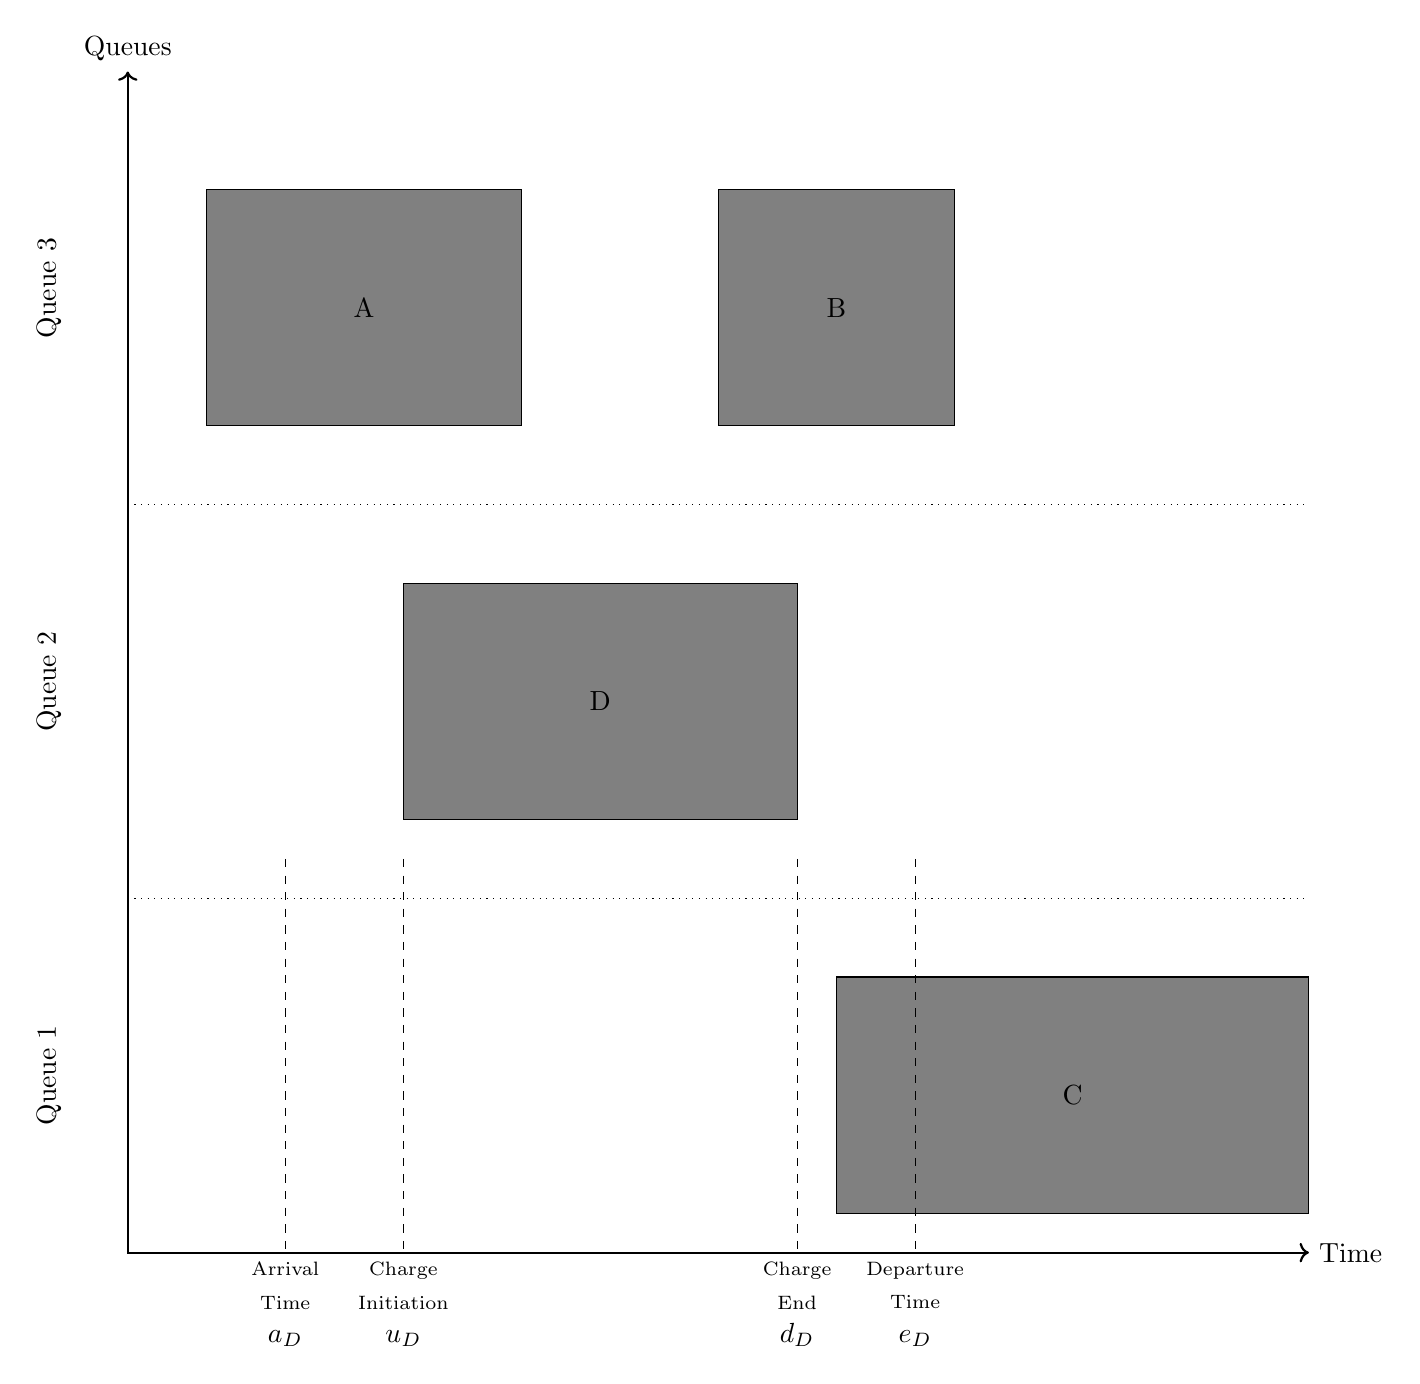
\begin{tikzpicture}
      % Variables
      \def \arrx   {2.0}
      \def \initx  {3.5}
      \def \endx   {8.5}
      \def \depx   {10.0}
      \def \yshift {5}

      % Axis
      \draw [thick,<->] (0,15) node[above]{Queues} -- (0,0) -- (15,0) node[right]{Time};

      % Rectangles
      \node[rectangle, draw, fill=gray, minimum width=4cm, minimum height = 3cm] at (3,12) {A};
      \node[rectangle, draw, fill=gray, minimum width=3cm, minimum height = 3cm] at (9,12) {B};
      \node[rectangle, draw, fill=gray, minimum width=5cm, minimum height = 3cm] at (6,7) {D};
      \node[rectangle, draw, fill=gray, minimum width=6cm, minimum height = 3cm] at (12,2) {C};

      % X-axis labels
      \node [below,align=center] at (\arrx,0) {\scriptsize Arrival     \\ \scriptsize Time \\ $a_D$};
      \node [below, align=center] at (\initx,0) {\scriptsize Charge    \\ \scriptsize Initiation  \\ $u_D$};
      \node [below, align=center] at (\endx,0) {\scriptsize Charge     \\ \scriptsize End \\ $d_D$};
      \node [below, align=center] at (\depx,0) {\scriptsize Departure  \\ \scriptsize Time \\ $e_D$};

      % Y-axis labels
      \node[rotate=90] at (-1, 2.25) {Queue 1};
      \node[rotate=90] at (-1, 7.25) {Queue 2};
      \node[rotate=90] at (-1, 12.25) {Queue 3};

      % Vertical lines
      \draw[dashed] (\arrx,\yshift)--(\arrx,0);
      \draw[dashed] (\initx,\yshift)--(\initx,0);
      \draw[dashed] (\endx,\yshift)--(\endx,0);
      \draw[dashed] (\depx,\yshift)--(\depx,0);

      % Horizontal lines
      \draw[dotted] (0, 4.5) -- (15, 4.5);
      \draw[dotted] (0, 9.5) -- (15, 9.5);

    \end{tikzpicture}
  }}
  \caption{Visualization of the temporal and spatial aspect of the aspect of the schedule. The grey rectangle labeled $D$ represents the time that the charger in queue 2 is active. $a_D$ represents the arrival time for bus $D$. The diagram indicates that $D$ arrives prior to the inital charge time, $u_D$. $d_D$ is the detatch time for bus $D$, which is before the departure time $e_D$. Physically, that represents bus $D$ being idle between $a_D$ and $u_D$ while its waiting to be charged, charging between $u_D$ and $d_D$, and idle again between $d_D$ and $e_D$ waiting to depart on the next route.}
  \label{fig:spacial-and-temporal-constr}
\end{figure}

Constraint \ref{seq:c4} states that the starting service time for bus \(j\), \(u_j\), must be greater than the starting time
of bus \(i\), \(u_i\), plus its service time, \(s_i\). The last term utilizes big-M notation to activate or deactivate the
constraint. A value of \(\sigma_{ij} = 1\) will activate the constraint to ensure that bus \(i\) is complete before bus \(j\) is
allowed to begin being serviced. If \(\sigma_{ij} = 0\), then the constraint is of the form \(T + u_j + s_j > u_i\) rendering the
constraint ``inactive'' because \(u_i\) cannot be larger than \(d_i\). This effectively allows the charging windows of the
vehicle to overlap.

Similarly, \(\phi_{ij}\) determines whether the vehicles will be charging in the same queue. If \(\phi_{ij} = 1\) then
\eqref{seq:c1} is rendered active and vehicle \(i\) and \(j\) must be charging in different queues. If \(\phi_{ij} = 0\) then the
constraint is deactivated and the vehicle queue assignments may be the same.

\ref{seq:c5} calculates the discharge for the route after visit \(i\). \ref{seq:c6} describes the service time of the bus.
\ref{seq:c7} calculates the initial charge for the next visit for bus \(b_i\). \ref{seq:c7} ensures that the bus is not
being over-charged. \ref{seq:c9} and \ref{seq:c10} are used to enable and disable the penalty method in \ref{eq:ac}. This is
done by checking if the initial charge for visit \(i\) is greater than or equal to the minimum allowed charge.
\ref{seq:c10} ensures the continuity of the times (i.e. the arrival time is less than the initial charge which is less
than the detach time which is less than the time the bus exits the station and all must be less than the time horizon).

The last set of constraints \ref{seq:c13} - \ref{seq:c17} set the rules for the decision variable \(\iota_h\). \ref{seq:c13}
and \ref{seq:c14} ensure that the initial charge time for visit \(i\), \(u_i\), is greater than the discrete time, \(0.25 \cdot
h\), being checked. Similarly, \ref{seq:c15} and \ref{seq:c16} ensure that the final charge time, \(d_i\), is less than the
next discrete time step, \(dt_h\). The final constraint \ref{seq:c17} is the discrete representation of whether charger
\(v_i \in \Qset\) is active.
\section{Simulated Annealing}
\label{sec:simulated-annealing}
SA is an exploitation oriented, single-solution based (as compared to population based) metaheuristic approach in which
its main advantage is its simplicity both theoretically and in its implementation as well its inherit ability to
overcome nonlinearities \cite{gendreau-2018-handb-metah,radosavljevic-2018-metah-optim}. This model is named after its
analogized process where a crystalline solid is heated then allowed to cool very slowly until it achieves its most
regular possible crystal lattice configuration \cite{henderson-1989-theor-pract}. There are five key components to SA:
initial temperature, cooling schedule (temperature function), generation mechanism, acceptance criteria, local search
iteration count (temperature change counter) \cite{keller-2019-multi-objec}.

\subsection{Cooling Equation (Experimental)}
\label{cooling-equation-experimental}
The initial temperature and cooling schedule are used to regulate the speed at which the solution attempts to converge
to the best known solution. When the temperature is high, SA encourages exploration. As it cools down (in accordance to
the cooling schedule), it begins to encourage local exploitation of the solution
\cite{rutenbar-1989-simul-anneal-algor,henderson-1989-theor-pract}]. There are three basic types of cooling equations
as shown in \ref{fig:cool} \cite{keller-2019-multi-objec}. The different types merely dictate the rate at which the algorithm
progressively disallows exploration. A linear cooling schedule is defined by \ref{eq:cool0}.

\begin{equation}
\label{eq:cool0}
\Tau[n] = \Tau[n-1] - \Delta_0
\end{equation}

with \(\Tau[0] = \Tau_0\) and \(\Delta_0 = 1/2\; C^\circ\) in \ref{fig:cool}. A geometric cooling schedule is mostly used in practice
\cite{keller-2019-multi-objec}. It is defined by \ref{eq:cool1}.

\begin{equation}
\label{eq:cool1}
\Tau[n] = \alpha \Tau[n-1]
\end{equation}

where \(\alpha = 0.995\) in \ref{fig:cool}. An Exponential cooling schedule is defined by the difference equation is defined as
\ref{eq:cool2}.

\begin{equation}
\label{eq:cool2}
\Tau[n] = e^{\beta}\Tau[n-1]
\end{equation}

where \(\beta = 0.01\) in \ref{fig:cool}. The initial temperature, \(T_0\), in the case of \ref{fig:cool}, is set to \(500^\circ\; C\) and
each schedule's final temperature is \(1\; C^\circ\).

\begin{figure}[htbp]
\centering
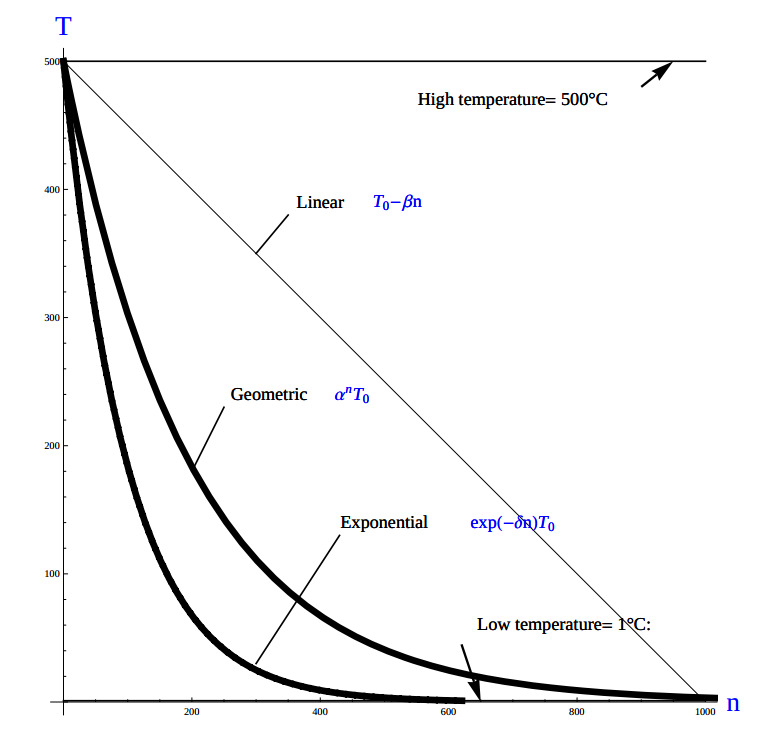
\includegraphics[width=0.5\textwidth]{sections/img/cool-func.jpg}
\caption{\label{fig:cool}Cooling equations}
\end{figure}

\subsection{Acceptance Criteria}
\label{sec:acceptance}
Acceptance criteria describes the method to accept or reject a given candidate solution. In SA, if a new candidate
solution is more fit than the currently stored solution it is always accepted as the new solution. However, within SA,
worse candidate solutions may be accepted as the new solution. The probability of accepting the candidate solution is
described by the function \(\exp(-\frac{J(x) - J(x')}{\Tau})\) where \(J(\cdot)\) is the objective functions described in
\ref{sec:objective-function}. The probability of acceptance is a function of the cooling equation just described and
difference of the current solution and a new candidate solution. Let \(\Delta E \equiv J(x) - J(x')\) where \(x\) is the current
solution and \(x'\) is the new candidate solution. The probability of acceptance of \(x'\) is defined by \ref{eq:candaccept}
\cite{keller-2019-multi-objec}.

\begin{equation}
\label{eq:candaccept}
f(x,x',T) =
\begin{cases}
  1                 & \Delta E > 0 \\
  e^{- \frac{\Delta E}{T}} & \text{otherwise}
\end{cases}
\end{equation}

\subsection{Generation Mechanisms}
\label{sec:generation-mechanisms}
Generation mechanisms in SA are used to generate random solutions to propose to the optimizer, these are known as
candidate solutions. In the case of the problem statement made in \ref{sec:problem-description}, five generation mechanism
shall be used: new visit, slide visit, new charger, remove, new window. The purpose of each of these generators is to
assign new visits to a charger, adjust a bus visits initial and final charge time within the same time frame/queue,
remove a bus from a charger, and place a bus visit into a new time slot/queue. Each generator will be discussed in more
detail in \ref{sec:generators}.

These generator mechanisms will in turn be utilized by two wrapper functions. The schedule generation is to used create
candidate solutions for SA to compare with other solutions, and the perturb schedule generator is used to take a
candidate solution and alter it slightly in an attempt to fall into a global/local minimum.

\subsubsection{Generator Input/Output}
\label{sec:generator-input-output}
This section discusses in detail the expected inputs and output of each generator. It is important to discuss these
parameters in order to have an understanding of the generating algorithms derived. The input consists of the bus visit
index of interest, information about the current state of arrivals, \(\I\), and the current state of the chargers'
availability, \(\C\). The output of each generator affects the tuple of decision variables \((v_i, u_i, d_i) \subset \I_i\).

\paragraph{Generator Input}
\label{sec:org2fa6d79}
Each generator has the tuple input of \(\Sol \equiv (i, \I, \C)\) where \(i\) is the visit index, \(\I_i\) is the tuple \(\visit\)
(\ref{sec:problem-description}), that describes the set of visits, and \(\C\) is the set that describes the availability for
all chargers \(q \in \Qset\). In other words, \(\C\) defines the set of times when the chargers are not being utilized or are
``inactive''.

To derive \(\C\), consider its inverse, \(\C'\), which is the set of ``active'' time periods for each charger, \(\C' = \bigcup
\{\C_q' : q \in \mathcal{Q}\}\) where \(\C_q' \subset \C'\) describes the active times for chagrer \(q\). Focusing on an individual charger,
consider \(\C_q'\) before a schedule has been imposed upon it, \(\C_q' \in \varnothing\). In other words, no buses have been
assigned to be charged over the time period of \([u_i, d_i]\). After the scheduling process is complete, \(\C_q'\) will have
a set of active periods of the form \(\C_q' \in \{[u_j, d_j]: j \in \Jsetq \}\) where \(\Jsetq \subset \mathcal{I}\). For \(\C_q'\) to be of
value, its compliment is to be found, \(\C_q\). Let \(j\text{th}\) inactive period shall be denoted as \(\C^j_q\).

To determine the inverse of \(\C_q'\), begin by noting \(\C_q' \bigcap \{[u_j, d_j] : j \in \Jsetq\} = \varnothing\), is said to be
disjoint \cite{halmos-1974-naive-set-theor}. The inverse of a disjoint set can be found by the De Morgan Law as shown
in \ref{eq:demorgan}. Using \ref{eq:demorgan}, the set of inactive periods can be written as \(\C_q \equiv \bigcup \{[u_j, d_j]': j \in \Jsetq\}\).
Let \(\Sol\) denote the tuple \(\Sol \equiv (i, \I, \C)\).

\begin{equation}
\label{eq:demorgan}
(A \cap B)' = A' \cup B'
\end{equation}

\paragraph{Generator Output}
\label{sec:org28269af}
The output is a modified visit, noted as \(\I_i'\). In actuality only the decision variables are being altered which is a
subset of \(\I_i\). Let this subset be defined by \(x_i' \equiv (v_i, u_i, d_i) \subset \I_i\) which is the chosen queue, initial
charge time, and detach time from the generator, \((v_i, u_i, d_i)\). The nature of SA implies that the generators have a
sense of randomness. Because of that, some of the generators may have multiple choices for what \(x_i'\) may be. Let the
set of candidates for the output be defined as \(x_i' \in X_i'\). Furthermore, set the set of candidate visits be denoted as
\(\I_i' \in \I'\).

\subsubsection{Generators}
\label{sec:generators}
This section describes and outlines the algorithm pool for the different generator types that are utilized in the
wrapper functions. Note that to satisfy constraints, \(B\) extra idle queues that provide no power to the bus. Because of
this, the set of queues is fully defined as \(q \in \{1,..., Q, Q+1,..., Q+B\}\) where \(Q\) is the total amount of chargers
and \(b\) is the bus ID. The use case for this is for when a bus is not to be placed on a charger, it will be placed in
the queue, \(v_i \in \{Q+1,..., Q+B\}\), which will satisfy the constraints above while allowing the bus to be ``set aside''
while others charge.

\paragraph{New visit}
\label{new-visit}
The new visit generator describes the process of moving bus \(b\) from the idle queue, \(v_i \in \{Q+1,..., Q+B\}\) to a valid
charging queue, \(v_i \in \{1,..., Q\}\). Lines 2-4 extracts the visit, \(i\), arrival time, \(a_i\), and departure time, \(e_i\).
Note that in subsequent algorithms these lines will be omitted for conciseness. Line 5 loops through the inactive time
periods that contain the time the bus is at the station, \([a_i, e_i]\). \(\U_{\cdot}\) indicates that an element is selected
randomly with a uniform distribution from the set \(\{\cdot\}\). Line 6 verifies that the inactive period selected is valid
and returns a random charging time, \([u_i, d_i]\), if it is. Line 7 returns the new visit.

\begin{algorithm}[H]
\caption{New visit algorithm} \label{alg:new-visit}
    \LinesNumbered
    \TitleOfAlgo{New Visit}
    \KwIn{($\Sol$)}
    \KwOut{$\I_i'$}

    \SetKwFunction{Union}{Union}
    \SetKwFunction{findFreeTime}{findFreeTime}

    \Begin
    {
        $i    \leftarrow \{i: i \in \Sol \}$ \tcc*{The index of the visit $i$}
        $a_i  \leftarrow \{ a_i \in \I_i : \I_i \in \I \subset \Sol \}$ \tcc*{Get the arrival time for visit $i$}
        $e_i  \leftarrow \{ e_i \in \I_i : \I_i \in \I \subset \Sol \}$ \tcc*{Get the departure time for visit $i$}

        \tcc{Randomly select a free time, $j$, from any charger $q \in \Qset$ that is within the time frame $[a_i e_i]$}
        \While {$C_q^j \in \{[a_i, e_i]\} \subset \U_{\C}$}
        {
            \If(\tcc*[f]{If there is time available in $C_q^j$}){$x_i' \leftarrow$ \findFreeTime{$C_q^j, (a_i, e_i)$} $\not\in \varnothing$}
            {
                \Return{$\I_i' \leftarrow x_i'$} \tcc*[f]{Return visit}
            }
        }
    }
\end{algorithm}

The function \texttt{findFreeTime} in \ref{alg:new-visit} is defined in \ref{alg:find-free-time}. \(L\) and \(U\) are the lower
and upper bound of the time between scheduled times. The possible use cases are depicted in \ref{fig:find-free}. In each case
depicted by \ref{fig:find-free}, the red line shows the arrival and departure time for an arbitrary bus visit, \(i\). The blue
lines indicate reigons in which charger \(q\) is active. \(C \in \C_q \subset \C\) represents one of the regions between the blue
lines, \([L, U]\) which stand for the lower and upper portions of the regions, respectively. The output of
\ref{alg:find-free-time}. That is, the only scheduling constraint is that the arrival time is before charger \(q\) is
available to charge the bus. Therefore, the bus must wait intil \(L\) before changer \(q\) may charge it. Furthermore, the
range that \(u_i\) must be selected from is \([L,e]\).

\begin{figure}
\centering
\begin{subfigure}{\textwidth}
    \centering
    \caption{Valid position: $a \leq u \leq d \leq e$}
    \label{subfig:sandwich}
    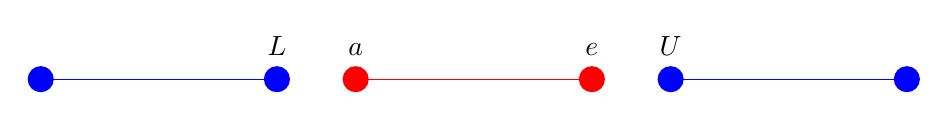
\begin{tikzpicture}[scale=2]
        \coordinate (A) at (0,0);
        \coordinate (B) at (1.5,0);
        \coordinate (C) at (2.0,0);
        \coordinate (D) at (3.5,0);
        \coordinate (E) at (4.0,0);
        \coordinate (F) at (5.5,0);

        \draw[blue] (A) -- (B);
        \draw[red]  (C) -- (D);
        \draw[blue] (E) -- (F);

        \node[circle,fill=blue,radius=0.15]                     at (A) {};
        \node[circle,fill=blue,radius=0.15,label=above : $L$]   at (B) {};
        \node[circle,fill=red,radius=0.15,label=above  : $a$] at (C) {};
        \node[circle,fill=red,radius=0.15,label=above  : $e$] at (D) {};
        \node[circle,fill=blue,radius=0.15,label=above : $U$]   at (E) {};
        \node[circle,fill=blue,radius=0.15]                     at (F) {};
    \end{tikzpicture}
\end{subfigure}

\par\bigskip

\begin{subfigure}{\textwidth}
    \centering
    \caption{Valid position: $L \leq u \leq d \leq e$}
    \label{subfig:all}
    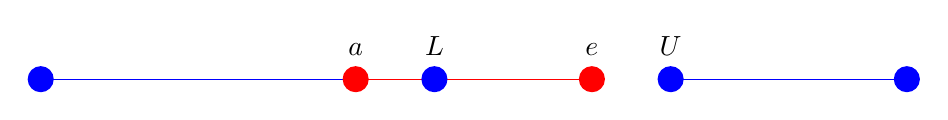
\begin{tikzpicture}[scale=2]
        \coordinate (A) at (0,0);
        \coordinate (B) at (2.5,0);
        \coordinate (C) at (2.0,0);
        \coordinate (D) at (3.5,0);
        \coordinate (E) at (4.0,0);
        \coordinate (F) at (5.5,0);

        \draw[blue] (A) -- (B);
        \draw[red]  (C) -- (D);
        \draw[blue] (E) -- (F);

        \node[circle,fill=blue,radius=0.15]                     at (A) {};
        \node[circle,fill=blue,radius=0.15,label=above : $L$]   at (B) {};
        \node[circle,fill=red,radius=0.15,label=above  : $a$] at (C) {};
        \node[circle,fill=red,radius=0.15,label=above  : $e$] at (D) {};
        \node[circle,fill=blue,radius=0.15,label=above : $U$]   at (E) {};
        \node[circle,fill=blue,radius=0.15]                     at (F) {};
    \end{tikzpicture}
\end{subfigure}

\par\bigskip

\begin{subfigure}{\textwidth}
    \centering
    \caption{Valid position: $a \leq u \le d \leq U$}
    \label{subfig:egu}
    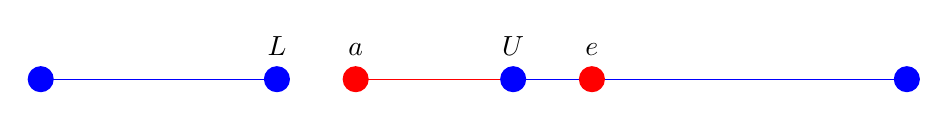
\begin{tikzpicture}[scale=2]
        \coordinate (A) at (0,0);
        \coordinate (B) at (1.5,0);
        \coordinate (C) at (2.0,0);
        \coordinate (D) at (3.5,0);
        \coordinate (E) at (3.0,0);
        \coordinate (F) at (5.5,0);

        \draw[blue] (A) -- (B);
        \draw[red]  (C) -- (D);
        \draw[blue] (E) -- (F);

        \node[circle,fill=blue,radius=0.15]                     at (A) {};
        \node[circle,fill=blue,radius=0.15,label=above : $L$]   at (B) {};
        \node[circle,fill=red,radius=0.15,label=above  : $a$] at (C) {};
        \node[circle,fill=red,radius=0.15,label=above  : $e$] at (D) {};
        \node[circle,fill=blue,radius=0.15,label=above : $U$]   at (E) {};
        \node[circle,fill=blue,radius=0.15]                     at (F) {};
    \end{tikzpicture}
\end{subfigure}

\par\bigskip

\begin{subfigure}{\textwidth}
    \centering
    \caption{Valid position: $L \le u \leq d \leq U$}
    \label{subfig:invertsandwhich}
    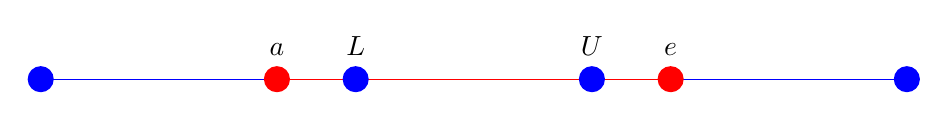
\begin{tikzpicture}[scale=2]
        \coordinate (A) at (0,0);
        \coordinate (B) at (1.5,0);
        \coordinate (C) at (2.0,0);
        \coordinate (D) at (3.5,0);
        \coordinate (E) at (4.0,0);
        \coordinate (F) at (5.5,0);

        \draw[blue] (A) -- (C);
        \draw[blue] (D) -- (F);
        \draw[red]  (B) -- (E);

        \node[circle,fill=blue,radius=0.15]                    at (A) {};
        \node[circle,fill=red,radius=0.15,label=above : $a$]   at (B) {};
        \node[circle,fill=blue,radius=0.15,label=above  : $L$] at (C) {};
        \node[circle,fill=blue,radius=0.15,label=above  : $U$] at (D) {};
        \node[circle,fill=red,radius=0.15,label=above : $e$]   at (E) {};
        \node[circle,fill=blue,radius=0.15]                    at (F) {};
    \end{tikzpicture}
\end{subfigure}

\par\bigskip

\begin{subfigure}{\textwidth}
    \centering
    \caption{Invalid position upper bound}
    \label{subfig:invalid-upper}
    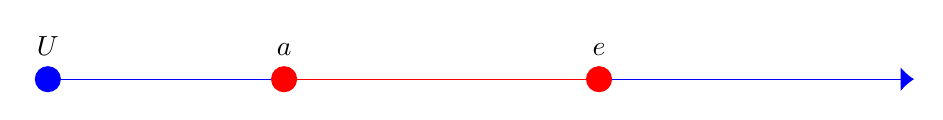
\begin{tikzpicture}[scale=2]
        \coordinate (A) at (0.0,0);
        \coordinate (B) at (5.5,0);
        \coordinate (C) at (1.5,0);
        \coordinate (D) at (3.5,0);

        \draw[-{Latex[width=3mm]},blue]  (A) -- (B);
        \draw[red]  (C) -- (D);

        \node[circle,fill=blue,radius=0.15,label=above : $U$] at (A) {};
        \node[circle,fill=red,radius=0.15,label=above  : $a$] at (C) {};
        \node[circle,fill=red,radius=0.15,label=above  : $e$] at (D) {};
    \end{tikzpicture}
\end{subfigure}

\par\bigskip

\begin{subfigure}{\textwidth}
    \centering
    \caption{Invalid position lower bound}
    \label{subfig:invalid-lower}
    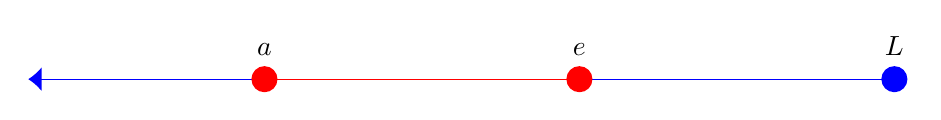
\begin{tikzpicture}[scale=2]
        \coordinate (A) at (0.0,0);
        \coordinate (B) at (5.5,0);
        \coordinate (C) at (1.5,0);
        \coordinate (D) at (3.5,0);

        \draw[-{Latex[width=3mm]},blue]  (B) -- (A);
        \draw[red]  (C) -- (D);

        \node[circle,fill=blue,radius=0.15,label=above : $L$] at (B) {};
        \node[circle,fill=red,radius=0.15,label=above  : $a$] at (C) {};
        \node[circle,fill=red,radius=0.15,label=above  : $e$] at (D) {};
    \end{tikzpicture}
\end{subfigure}

\caption{Outlines the different cases that requested time and charger allocated time can overlap}
\label{fig:find-free}
\end{figure}

\begin{algorithm}[H]
\caption{Find free time algorithm searches and returns the available time frames} \label{alg:find-free-time}
    \LinesNumbered
    \TitleOfAlgo{Find Free Time}
    \KwIn{$(L,U,a,e)$}
    \KwOut{$(u,d)$}

    \Begin
    {
        \If(\tcc*[f]{If $L < a < e < U]$ (\autoref{subfig:sandwich})}){$L \leq a$ and $U \geq e$}
        {
                u $\leftarrow$ $\U_{[a,e]}$\;
                d $\leftarrow$ $\U_{[u,e]}$\;
        }
        \ElseIf(\tcc*[f]{Else if $a < L < e < U$ (\autoref{subfig:all})}){$L > a$ and $U \geq e$}
        {
                u $\leftarrow$ $\U_{[L,e]}$\;
                d $\leftarrow$ $\U_{[u,e]}$\;
        }
        \ElseIf(\tcc*[f]{Else if $L < a < U < e$ (\autoref{subfig:egu})}){$L \leq a$ and $U < e$}
        {
                u $\leftarrow$ $\U_{[a,U]}$\;
                d $\leftarrow$ $\U_{[u,U]}$\;
        }
        \ElseIf(\tcc*[f]{Else if $a \leq u \leq d \leq L$ or $U \leq a \leq d \leq e$ (\autoref{subfig:invertsandwhich})}){$L > a$ and $U < e$}
        {
                u $\leftarrow$ $\U_{[a,L], [U,e]}$\;
                d $\leftarrow$ $\U_{[u,L], [u,e]}$\;
        }
        \Else(\tcc*[f]{Otherwise the bus cannot be scheduled in this time frame (\autoref{subfig:invalid-lower}, \autoref{subfig:invalid-upper})})
        {
                u $\leftarrow$ $\varnothing$\;
                d $\leftarrow$ $\varnothing$\;
        }

        \Return{(u,d)}
    }
\end{algorithm}

\paragraph{Slide visit}
\label{slide-visit}
Slide visit (\ref{alg:slide-visit}) is used for buses that have already been scheduled. Because of the constraint
\ref{seq:c10} there may be some room to move \(u_i\) and \(d_i\) within the window \([a_i, e_i]\). Two new values, \(u_i\) and
\(d_i\) are selected with a uniform distribution to satisfy the constraint \(a_i \leq u_i \leq d_i \leq e_i\). Line 2 randomly loops
through the other inactive time frames from charger \(v_i\) that is within the time that the bus is at the station, \([a_i,
e_i]\). Line 3 verifies the time frame previously selected and returns a new charging time. Line 4 returns the new visit.

\begin{algorithm}[H]
\caption{Slide Visit Algorithm} \label{alg:slide-visit}
    \LinesNumbered
    \TitleOfAlgo{Slide Visit}
    \KwIn{$\Sol$}
    \KwOut{$\I_i'$}

    \Begin
    {
        \tcc{Randomly select an inactive time frame, $j$, from charger $v_i$ that is within the time frame $[a_i, e_i]$}
        \While {$C_q^j \in \{[a_i, e_i]\} \subset \U_{\C_{v_i}}$}
        {
            \If(\tcc*[f]{If there is time available in $C_q^j$}){$x_i' \leftarrow$ \findFreeTime{$C_q^j$, ($a_i, e_i$)} $\not\in \varnothing$}
            {
                \Return{$\I_i \leftarrow x_i'$} \tcc*[f]{Return visit}
            }
        }
    }
\end{algorithm}

\paragraph{New charger}
\label{new-charger}
The new charger generator takes a visit \(\I_i\) and changes the charger it is on while maintianing the same charge time,
\([u_i, d_i]\). Similar to \ref{alg:new-visit}, the new candidate, \(x_i'\), must be checked before being added to the set \(X_i'\).
Line 2 randomly loops through any time frame from any charger, \(C_q^j\), that is within the time frame that the bus is at
the station, \([a_i, e_i]\). Line 3 verifies the selection and line 4 returns the new visit.

\begin{algorithm}[H]
\caption{New Charger Algorithm} \label{alg:new-charger}
    \LinesNumbered
    \TitleOfAlgo{New Charger}
    \KwIn{$\Sol$}
    \KwOut{$\I_i'$}

    \Begin
    {
        \tcc{Randomly select an inactive time frame, $j$, from any charger $q \in \Qset$ that is within the time frame $[a_i, e_i]$}
        \While {$C_q^j \in \{[a_i, e_i] \} \subset \U_{\C}$}
        {
            \If (\tcc*[f]{If the charge time is within the region $[L,U]$}) {$L \leq u_i$ \And $U \geq d_i$}
            {
                \Return{$\I_i \leftarrow x_i'$} \tcc*[f]{Return visit}
            }
        }

    }
\end{algorithm}

\paragraph{Remove}
\label{sec:remove}
The remove generator simply removes a bus from a charger queue and places it in its idle queue, \(v_i \in
\{Q,...,Q+B\}\).

\begin{algorithm}[H]
\caption{Remove algorithm} \label{alg:remove}
    \LinesNumbered
    \TitleOfAlgo{Remove}
    \KwIn{$\Sol$}
    \KwOut{$\I_i'$}

    \Begin
    {
       \Return{$\I_i' \leftarrow (Q+b,a_i,e_i)$}
    }
\end{algorithm}

\paragraph{New Window}
\label{sec:new-visit}
New window is a combination of the remove and then new visit generators (\ref{sec:remove} and \ref{sec:new-visit}). By this it is
meant that current scheduled tuple \((v_i, u_i, d_i)\) is removed and added back in as if it were a new visit.

\begin{algorithm}[H]
\caption{New window algorithm}
    \LinesNumbered
    \TitleOfAlgo{New Window}
    \KwIn{$\Sol$}
    \KwOut{$\I_i'$}

    \Begin
    {
        \SetKwFunction{NewVisit}{NewVisit}
        \SetKwFunction{Remove}{Remove}

        $\I_i' \leftarrow$ \Remove{$v,u,d$}   \tcc*{Remove visit $i$ from its charger}
        $\Sol \leftarrow \I_i'$               \tcc*{Update the route information tuple}
        $\I_i' \leftarrow$ \NewVisit{$\Sol'$} \tcc*{Add visit $i$ back in randomly}

        \Return{$(v,u,d)$}
    }
\label{alg:new-window}
\end{algorithm}

\subsubsection{Generator Wrappers}
\label{generator-wrappers}
This section covers the algorithms utilized to select and execute different generation processes for the SA process. The
generator wrappers are the method immediately called by SA. Each wrapper utilizes the generators previously described
and returns either metadata about the bus routes or a new valid charger schedule.

\paragraph{Schedule Generation}
\label{schedule-generation}
The objective of this generator is to generate a candidate solution to the given schedule. To generate a candidate
solution, the generator is given \(\I\), a bus is picked at random, \(b \in \Bset\), then a random visit is picked. The new
visit generator (\ref{alg:new-visit}) is then utilized. This process is repeated for each visit. This algorithm is
summarized in \ref{alg:schedule-generation}. Recall from \ref{sec:input-variables}, \(\Jset_B \subset \I\) is used to indicate the
set of visit indices for bus \(b\).

\begin{algorithm}[H]
\caption{Schedule generation algorithm} \label{alg:schedule-generation}
    \LinesNumbered
    \TitleOfAlgo{ScheduleGeneration}
    \KwIn{$\I$, $\C$}
    \KwOut{$\I'$, $\C'$}

    \SetKwFunction{Union}{Union}
    \SetKwFunction{NewVisit}{NewVisit}
    \SetKwFunction{UpdateQueues}{UpdateQueues}

    \Begin
    {
        $\I' \leftarrow \; \varnothing$\;
        \For {$\I_i' in \I$}
        {
            $b \leftarrow\; \U_{\Bset}$ \tcc*{Randomly select a bus with uniform distribution}
            $i\leftarrow\; \U_{\Jset_b}$ \tcc*{Randomly select a visit from bus $b$ with uniform distribution}
            $\I_i' \leftarrow \NewVisit{(visit.a, visit.e)}$ \tcc*{Assign the bus to a charger}
            \UpdateQueues{($\I_i'$, $\C_q$)} \tcc*{Update $\C_q$ with information in $I_i'$}
        }
            \Return{$\I'$, $\C'$}
    }
\end{algorithm}

\paragraph{Perturb Schedule}
\label{tweak-schedule}
As described in SA, local searches are also employed to try and exploit a given solution
\cite{radosavljevic-2018-metah-optim}. The method that will be employed to exploit the given solution is as follows:
pick a bus, pick a visit, pick a generator. The algorithm is outlined in \ref{alg:perturb-schedule}.

\begin{algorithm}[H]
\caption{Perturb schedule algorithm}

    \LinesNumbered
    \TitleOfAlgo{PerturbSchedule}
    \KwIn{$\I$, $\C$}
    \KwOut{$\I_i'$, $\C'$}

    \SetKwFunction{GeneratorCallback}{GeneratorCallback}

    \Begin
    {
        $b \leftarrow\; \U_{\Bset}$ \tcc*{Randomly select a bus with uniform distribution}
        $i\leftarrow\; \U_{\Jset_b}$ \tcc*{Randomly select a visit from bus $b$ with uniform distribution}
        $G \leftarrow\; \U_{[1,G_size]}$ \tcc*{Select one of the generator functions}
        $\I_i', \C' \leftarrow$ \GeneratorCallback{($G$, $j, \I, \C$)} \tcc*{Excecute the generator function}
        \UpdateQueues{($\I_i'$, $\C_q$)} \tcc*{Update $\C_q$ with information in $I_i'$}
        \Return{$\I'$, $\C$}
    }
\label{alg:perturb-schedule}
\end{algorithm}
\section{Optimization Algorithm}
\label{optimization-algorithm}
This final section combines the generation algorithms and the optimization problem into a single algorithm. It begins
with an introduction to a general SA algorithm which will be used to springboard into the construction of the SA PAP
algorithm. For the case of the pseudo SA algorithm to be presented, the notation pesented will be self-contained and not
related to any of the variables presented for SA PAP thus far. Consider \ref{alg:sa-pseudo} \cite{henderson-1989-theor-pract}.
\(\omega\) and \(\omega'\) are the current solution and the candidate solution, respectively. \(t_k\) is the temperature cooling
schedule, \(T\) is the initial temperature that will iterate until \(k = K\). \(M_k\) is the repetition counter, it defines
the number of iterations to execute for each temperture \(t_k\).

The algorithm behaves as follows: initialize the SA algorithm with an initial solution, temperature schedule, and
repetition schedule. The first loops until \(T = t_K\), the second loop finished whin \(m = M_k\). For each loop, create a
new solution, calculate the difference in the fitness of \(\omega\) and \(\omega'\). Update \(\omega\) with \(\omega'\) if the candidate solution is
better. Update \(\omega\) with \(\omega'\) with probability \(e^{\frac{-\Delta_{\omega , \omega'}}{t_k}}\) if the candidate solution is worse than the
current solution. This is repeated until the stopping criteria is met.

\begin{algorithm}[H]
\caption{Pseudo-code for SA} \label{alg:sa-pseudo}
    \LinesNumbered
    \TitleOfAlgo{SA Pseudo-Code}

    \SetKwFunction{f}{f}
    \Begin
    {
        $\omega \in W$ \tcc*{Select an initial solution}
        $k=0$ \tcc*{Select the temperature change counter}
        $t_k$ \tcc*{Select a temperature cooling schedule}
        $T = t_0 \geq 0$ \tcc*{Select an initial temperature}
        $\forall q \in \Qset : \C_q \in \{[0,T]\}$ \tcc*{Set the initial inactive time for each charger to the time horizon}
        \tcc{Select a repetition schedule $M_k$, that defines the number of iterations executed at each temerature $t_k$}

        \While{Stopping criterion not met}
        {
            $m \rightarrow 0$ \tcc*{Set repetition counter}
            \While{$m = M_k$}
            {
                $\omega' \in N(\omega)$ \tcc*{Generate a new solution}
                $\Delta_{\omega,\omega'} \rightarrow$ \f{$\omega'$} - \f{$\omega$} \tcc*{Calculate the difference of fitness scores}
                \If{$\Delta_{\omega , \omega'} \le 0$}{$\omega \rightarrow \omega'$}
                \If{$\Delta_{\omega , \omega'} > 0$}{$\omega \rightarrow \omega'$ with probability $e^{\frac{-\Delta_{\omega , \omega'}}{t_k}}$}
                $m \rightarrow m+1$\;
            }

        $k \rightarrow k+1$\;
        }
    }
\end{algorithm}

The objective now is to outline SA-PAP in \ref{alg:sa-pap}. Lines 2-4 initialize the SA algorithm by defining the initial
temperature, selecting the cooling schedule, and setting the repetition schedule. Line 5 loops through each of the step
in the temperature schedule \(\Tau \in \{ \Tau_0, \Tau_1, ..., \Tau_m \}\). Lines 6 and 7 generate a new solution and
calculates its fitness. \(\nu\) in this context is defined as \(\nu = (u, d, v, \eta)\) Lines 8 through 13 updates the solution
depending on if the new solution is better or worse than the previous solution. Line 14 iterates through the repetition
schedule, \(k \in \{1, 2, ..., K\}\). Lines 15-23 perturbs the previously generated solution, calculates its fitness, and
updates the current solution with the candidate solution depending on the fitness.

\begin{algorithm}[H]
\caption{Simulated annealing approach to the position allocation problem} \label{alg:sa-pap}
    \LinesNumbered
    \TitleOfAlgo{SA PAP}
    \KwIn{$\I$}
    \KwOut{$\I'$}

    \SetKwFunction{CoolingEquation}{CoolingEquation}
    \SetKwFunction{ScheduleGeneration}{ScheduleGeneration}
    \SetKwFunction{PerturbSchedule}{PerturbSchedule}
    \SetKwFunction{J}{J}

    \Begin
    {
        $\Tau_0$ \tcc*{Initialize temperature}
        $\Tau_{M} \leftarrow$ \CoolingEquation{$\Tau_0$} \tcc*{Select cooling equation}
        $K$ \tcc*{Set a repetition schedule}

        \For{$\Tau_m \in \{\Tau_0, \Tau_1, ..., \Tau_M\}$}
        {
            $\upsilon' \in Y \leftarrow$ \ScheduleGeneration{$\I$} \tcc*{Generate a new solution}
            $\Nu_{\upsilon, \upsilon'} = $ \J{$\upsilon'$}  - \J{$\upsilon$} \tcc*{Calculate the difference of fitness scores}
            \If{$\Nu_{\upsilon, \upsilon'} \le 0$}{$\upsilon \leftarrow \upsilon'$}
            \If{$\Nu_{\upsilon, \upsilon'} \le 0$}{$\upsilon \leftarrow \upsilon'$ with probability $e^{\frac{\Nu_{\upsilon, \upsilon'}}{\Tau_m}}$}

            \For{$k \in \{1, 2, ..., K\}$}
            {
                $\upsilon' \in Y \leftarrow$ \PerturbSchedule{$\I$} \tcc*{Perturb the solution and reassess}
                $\Nu_{\upsilon, \upsilon'} = $ \J{$\upsilon'$}  - \J{$\upsilon$} \tcc*{Calculate}
                \If{$\Nu_{\upsilon, \upsilon'} \le 0$}{$\upsilon \leftarrow \upsilon'$}
                \If{$\Nu_{\upsilon, \upsilon'} \le 0$}{$\upsilon \leftarrow \upsilon'$ with probability $e^{\frac{\Nu_{\upsilon, \upsilon'}}{\Tau_m}}$}
            } % For k
        }     % For \Tau
    }         % Begin
\end{algorithm}

\bibliographystyle{plain}
\bibliography{/home/alex/Documents/docs/sa-pap/citation-database/lit-ref,/home/alex/Documents/docs/sa-pap/citation-database/lib-ref,~/Documents/citation-database/lit-ref,~/Documents/citation-database/lib-ref}
\end{document}